\documentclass[a4paper,12pt]{report}

\usepackage[utf8]{inputenc}
\usepackage[russian]{babel}
\usepackage{amsmath}
\usepackage{multicol}
\setlength{\columnsep}{1cm}
\inputencoding{utf8}
\usepackage{graphicx}
\graphicspath{{images/}}

\usepackage{geometry} % Меняем поля страницы
\geometry{left=2cm}% левое поле
\geometry{right=1.5cm}% правое поле
\geometry{top=3cm}% верхнее поле
\geometry{bottom=2cm}% нижнее поле

\begin{document}

\begin{center}
\Large
{\bf Решение задачи №5 по анализу временных рядов.} 
{ Мазурин Константин.}
\end{center}

\underline{Постановка задачи:} Дан временной ряд $x_k = x({\Delta}tk)$, $k = 0,1,...,2N - 1$, у которого первое и второе, третье и четвертое и т.д. значения
попарно совпадают. Требуется доказать аналитически, что периодограмма такого ряда будет симметрична относительно частоты $\nu = 0.5\nu_c = 1/4{\Delta}t$.
Также следуюет проиллюстрировать это свойство с помощью программы СКАВРя.

Будет использоваться следующий ряд:
\begin{equation}
\overline{x}_k = A_{1}cos(2\pi\nu_{1}t_k - \phi_1) + A_{2}cos(2\pi\nu_{2}t_k - \phi_2) + \sigma_{x}\xi_k 
\end{equation}
\begin{equation}
t_k = {\Delta}t k; \hspace{2cm} k = 0,1,2,...,N-1
\end{equation}
Где ${\Delta}t$ - постоянный шаг выборки;
\\ $Ai, \nu_i, \phi_i, i = 1,2$ - амплитуды, частоты и фазы двух гармонических компонентов;
\\ $\xi_k$ - случайные величины с нулевым математическим ожиданием и единичной дисперсией, распределенные по нормальному закону (шумовой компонент ряда);
\\ $\sigma_x$ - среднеквадратическое отклонение шумового компонента, которое можно вычислить через отношение "сигнал к шуму" $\gamma$ с помощью соотношения
\begin{equation}
\sigma_x = \sqrt{\frac{A_{1}^2 + A_{2}^2}{2\gamma}}
\end{equation}
Для того, чтобы ряд подходил под условия задачи, каждый член ряда возьмем дважды, тем самым увеличив их количество до $2N$ и уменьшив вдвое шаг ряда ${\Delta}t$.

\vspace{1cm}
\underline{Решение:}
Для начала получим выражение для периодограммы ряда:
\begin{equation}
X_j = \sum\limits_{k=0}^{2N-1} x_{k}e^{-i\frac{2\pi}{2N}kj} = \sum\limits_{k=0}^{N-1} \overline{x}_{k}e^{-i\frac{2\pi}{N}kj} (1 + e^{-i\frac{2\pi}{2N}j}) 
= (1 + e^{-i\frac{2\pi}{2N}j}) \sum\limits_{k=0}^{N-1} \overline{x}_{k}e^{-i\frac{2\pi}{N}kj}
\end{equation}
\begin{equation}
D_j = \frac{1}{N^2} \lbrack Re^{2}X_j + Im^{2}X_j \rbrack = \frac{1}{N^2} \vert X_j \vert^2 = \frac{1}{N^2} \big\vert 1 + e^{-i\frac{2\pi}{2N}j} \big\vert^2 *
\Big\vert \sum\limits_{k=0}^{N-1} \overline{x}_{k}e^{-i\frac{2\pi}{N}kj} \Big\vert^2
\end{equation}
\begin{equation}
j = 0,1,...,N
\end{equation}

Мы видим, что последний множитель является периодограммой исходного ряда $\overline{x}_k$, построенной на первых $N$ точках. Также заметим, что частота $1/4{\Delta}t = 0.5\nu_c$
является Найквистовой для ряда $\overline{x}_k$. Из этих фактов следует, что частоты, отраженные на периодограмме, будут вдвое меньше, чем у исходного ряда.
Рассмотрим центральный множитель:
\begin{equation}
\big\vert 1 + e^{-i\frac{2\pi}{2N}j} \big\vert^2 = \big\vert 1 + \cos{\frac{2\pi}{2N}j} - i\sin{\frac{2\pi}{2N}j} \big\vert^2 = (1 + \cos{\frac{2\pi}{2N}j})^2 + \sin^2{\frac{2\pi}{2N}j} = 
2 + 2\cos{\frac{2\pi}{2N}j}
\end{equation}
Можно легко убедиться, что он будет c точностью до знака косинуса симметричен относительно $j = N/2$, что соответствует частоте $0.5\nu_c$. 

Также нетрудно показать, что и последний множитель примет одинаковые значения при $j$ и $N-j$, что говорит о симметрии относительно точки $j = N/2$.
\begin{equation}
\Big\vert \sum\limits_{k=0}^{N-1} \overline{x}_{k}e^{-i\frac{2\pi}{N}k(N-j)} \Big\vert^2 = \Big\vert \sum\limits_{k=0}^{N-1} \overline{x}_{k}e^{-i2\pi{k}}e^{i\frac{2\pi}{N}kj} \Big\vert^2 = 
\Big\vert \sum\limits_{k=0}^{N-1} \overline{x}_{k}e^{i\frac{2\pi}{N}kj} \Big\vert^2 = \Big\vert \sum\limits_{k=0}^{N-1} \overline{x}_{k}e^{-i\frac{2\pi}{N}kj} \Big\vert^2
\end{equation}

\newpage

\begin{center}
{\bf Результаты работы программы СКАВРя}
\end{center}
\begin{figure}[h]
\center{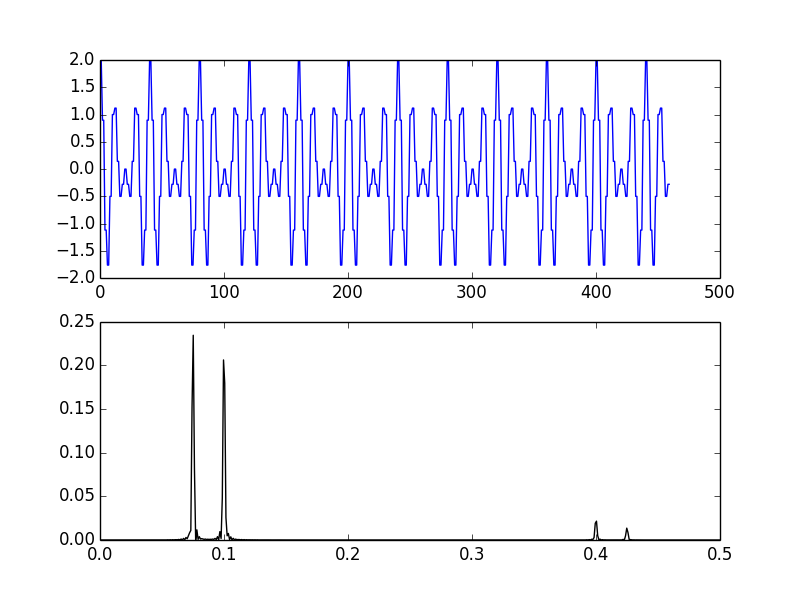
\includegraphics[width=1\linewidth]{figure_1.png}}
\caption{Временной ряд (сверху) и его периодограмма (снизу). $A_i = 1, \nu_1 = 0.2, \nu_2 = 0.15, \phi_i = 0$ }
\end{figure}

\end{document}

